% Chapter 11

\chapter{Diseño Experimental} % Write in your own chapter title
\label{Chapter11}
\lhead{Capítulo 11. \emph{Diseño Experimental}} % Write in your own chapter 

Basado en el diseño del Capítulo \ref{Chapter9}, se desarrollan las siguientes actividades con el objetivo de encontrar el mejor resultado para la implementación buscada; en este caso, un sistema embebido capaz de operar concurrentemente con un sistema operativo que se encargue de gestionar una conexión de red hacia la nube.

Se usa como banco de pruebas la tarjeta de desarrollo ZYBO con la distribución de Petalinux 2017.4 con Kernel de Linux versión 4.9.0 y File System por defecto de Petalinux 2017.4.
 
 \begin{itemize}
 
  \item Se analizan los tiempos de ejecución del código a implementar en Hardware junto con la versión Software mediante un Benchmark. Este medirá el tiempo de ejecución a lo largo de tres iteraciones; en el caso del HW, se medirá el rendimiento del mismo a las frecuencias de 100MHz y 150MHz, pudiendo así determinar la eficiencia del circuito.
 
 \item Se analizarán los tiempos de ejecución del Hardware a lo largo de 4 estrategias de optimización obtenidas mediante HLS así como la cantidad de recursos usados en cada solución.
 
 \item Se analizará el circuito con mejor rendimiento contra él mismo, modificando la estrategia de síntesis a una de optimización de área buscando reducir la cantidad de recursos usados por la solución.
 
 \item Finalmente se determina la relación rendimiento contra uso de recursos buscando la eficiencia más alta.
 
 \item Se determinará la ganancia SW vs HW; posteriormente, se analizará la viabilidad de la implementación en campo.
 
 \end{itemize}
 
La conexión entre el computador y la tarjeta de desarrollo se realiza dentro de una red local usando un enrutador de red como intermediario \ref{fig:router}. La manipulación de la consola de Linux se realiza usando PuTTY y la manipulación de los archivos de configuración se realiza usando un cliente SFTP con FileZilla. 

\begin{figure}[H]
	\centering
		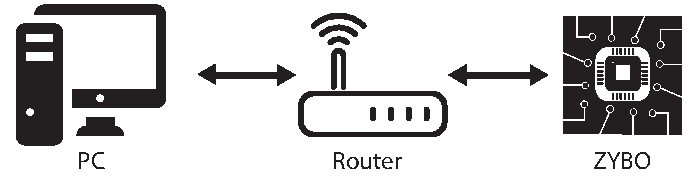
\includegraphics[scale=1]{./Figures/router.pdf}
	\caption{Esquema de conexión}
	\label{fig:router}
\end{figure}
